\chapter{Theorie}
\label{theory}

\todo[inline]{Warum Einigungsalgorithmus?}
\todo[inline]{FLP-Theorem}

\section{Crash-Recovery-Modell}

Alle in dieser Arbeit vorgestellten Einigungsalgorithmen basieren auf dem \textit{Crash-Recovery-Modell}. Server können abstürzen und nach einem Neustart wieder am Cluster teilnehmen. Außerdem kann das Netzwerk unzuverlässig sein. Nachrichten können also beliebig viel Zeit von einem Knoten zu einem anderen Knoten benötigen, verloren gehen oder die Reihenfolge ändern. Ziel dabei ist, dass der Einigungsalgorithmus solange eine Einigung erzielen kann, wie eine Mehrheit der Server funktioniert und erreichbar ist. Die teilnehmenden Server dürfen sich jedoch nicht beliebig falsch verhalten, also keine falschen Nachrichten schicken und keine Systemzustände erreichen, die nicht vorgesehen sind. Es gibt auch Einigungsalgorithmen, die gegen solche byzantinischen Fehler geschützt sind \cite{byzantine-paxos}, jedoch erhöht dies die Komplexität deutlich und es werden im Vergleich zum Crash-Recovery-Modell mehr Server benötigt, um sich vor der gleichen Anzahl an fehlerhaften bzw. ausfallenden Servern zu schützen.

\section{Einigungsalgorithmen}

\subsection{Paxos}

Der bekannteste Einigungsalgorithmus ist Paxos \cite{paxos, simple-paxos}. Paxos implementiert eine \textit{Replicated State Machine}. \todo[inline]{Grafik zur Replicated State Machine} Bei diesem Modell besitzt jeder Knoten eine Zustandsmaschine, die Befehle ausführt und dadurch den Zustand ändert. Der Einigungsalgorithmus kümmert sich darum, dass die Befehle auf allen Knoten in der gleichen Reihenfolge durchgeführt werden, sodass der Zustand auf allen Knoten konsistent ist.

Die einfache Version von Paxos (\textit{Basic Paxos}) ermöglicht die Einigung auf einen einzelnen Wert. Dabei werden die Teilnehmer in drei Rollen aufgeteilt:
\begin{itemize}
	\item Die \textbf{Acceptors} hören auf vorgeschlagene Werte, speichern diese und akzeptieren sie, falls sie nicht schon einen konfligierenden Wert akzeptiert haben.
	\item Der \textbf{Proposer} schlägt einen Wert vor, auf den sich geeinigt werden soll. Er sendet diese an die Acceptors.
	\item Die \textbf{Learner} erhalten den Wert, auf den sich geeinigt wurde und können entsprechend handeln, z.B. indem sie eine Antwort an einen Client senden.
\end{itemize}

Die Einigung auf einen Wert erfolgt in zwei Phasen:

\begin{enumerate}
	\item 
		\begin{enumerate}[label=\alph*)]
			\item Der Proposer wählt eine Proposal Number \textit{n} und sendet sendet eine eine Prepare-Nachricht mit  \textit{n} an die Acceptors. 
			\item Die Acceptors akzeptieren \textit{n}, falls sie noch keine Proposal Number akzeptiert haben, die größer als \textit{n} ist. Sie antworten mit der höchsten Proposal Number, die sie akzeptiert haben.
		\end{enumerate}
	\item
		\begin{enumerate}[label=\alph*)]
		\item Wenn der Proposer von einer Mehrheit der Acceptors eine Antwort auf seine Prepare-Nachricht mit der Proposal Number \textit{n}] erhalten hat, sendet er eine Accept-Nachricht an die Acceptors mit \textit{n} und einem Wert \textit{v}, auf den sich geeinigt werden soll.
		\item Die Acceptors akzeptieren den vorgeschlagenen Wert \textit{v} mit der Proposal Number \textit{n}, falls sie noch nicht auf eine Prepare-Nachricht mit höherer Proposal Number geantwortet haben.
	\end{enumerate}
\end{enumerate}

Um sich auf beliebig viele Werte zu einigen, werden beliebig viele Paxos-Instanzen hintereinander ausgeführt (\textit{Multi-Paxos} \cite{paxos-made-live}). Dabei können mehrere Optimierungen vorgenommen werden. Da sich mehrere Proposer gegenseitig behindern würden und das System u.U. dann häufig keine Einigung erzielen könnte, sollte im Normalbetrieb nur ein einzelner Proposer vorhanden sein. Dieser kann durch einen beliebigen Leader-Election-Algorithmus gewählt werden. Falls dieser ausfällt, muss ein neuer Proposer gewählt werden. Es ist jedoch kein Problem, falls es zu einem Zeitpunkt mehrere Leader geben sollte, da Paxos dann garantiert, dass keine unterschiedlichen Werte akzeptiert werden. Dies sollte jedoch nicht die Regel sein. Außerdem kann der Leader die Phase 1 einmalig für beliebig viele Werte durchführen, wodurch sich die Nachrichtenanzahl reduziert.

In Implementierungen wird meist eine Client-Server-Architektur verwendet. Dabei übernehmen die Server alle drei Rollen. Die Clients senden (Lese- und Schreib-)Anfragen an das System und bekommen die Werte zurück, auf die sich geeinigt wurde, ähnlich einer Datenbank.

Paxos wurde bereits in anderen Arbeiten implementiert \cite{paxos-made-code, paxos-made-live}. Die Autoren berichten jeweils von nicht-trivialen Problemen, auf die sie während der Arbeit an einer Implementierung gestoßen sind. Dafür mussten sie unter anderem Optimierungen vornehmen, die nicht in der initialen Beschreibung des Algorithmus enthalten sind. Außerdem gibt es sehr wenige Implementierungen, insbesondere welche die Open-Source sind.

\subsection{Zookeeper/Zab}

\todo[inline]{Kerneigenschaften genau formulieren, eigene Grafik zum Paxos Randfall erstellen}

Zookeeper implementiert einen Algorithmus namens Zab \cite{zab}. Zab ist ebenfalls ein Einigungsalgorithmus, der jedoch leicht andere Garantien bietet. Die Autoren nennen ihr Modell ein \textit{Primary-Backup System}. Es gibt zu jedem Zeitpunkt höchstens einen Primary-Server, der Vorschläge für den nächsten Befehl an die anderen Server im Cluster senden kann. Die anderen Server sind exakte Backup-Replikate des Primary-Servers. Falls der Primary-Server ausfällt, wird eine neuer Primary-Server aus den vorhandenen Backup-Servers gewählt. Die Autoren erklären den Unterschied zu Paxos so: Zab soll garantieren, dass jede Zustandsänderung von allen vorherigen Zustandsänderungen abhängt und somit niemals vor diesen ausgeführt werden darf. Außerdem sollen von einem Proposer mehrere Befehle, hier Transaktionen genannt, einzeln und nebenläufig vorgeschlagen werden können, ohne dass sich ihre Reihenfolge ändern kann. Paxos kann in diesem Randfall jedoch nicht die initiale Reihenfolge garantieren (siehe Abbildung \ref{fig:paxos_fail}).

\begin{figure}[H]
	\centering
	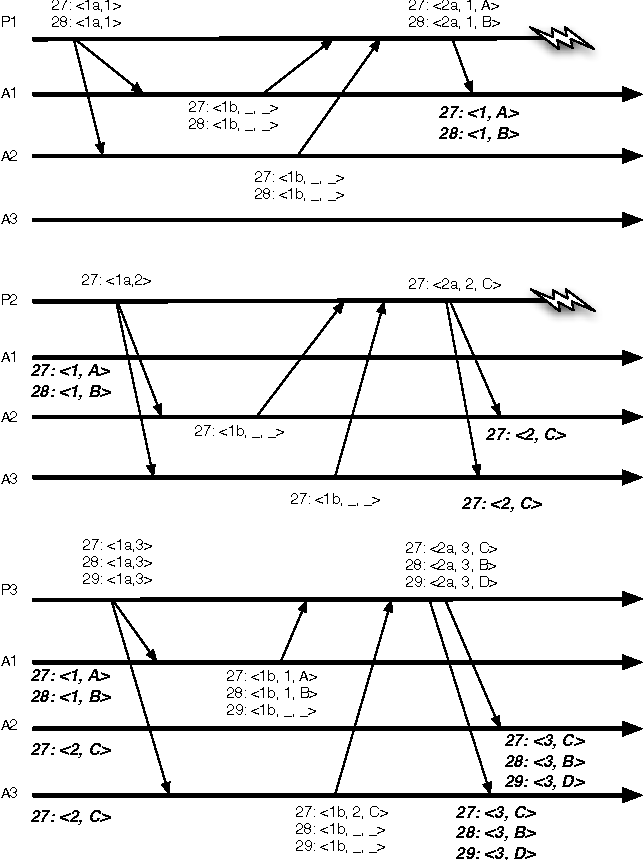
\includegraphics[height=350px]{img/paxos_fail.png}
	\caption{Randfall von Paxos, bei dem sich die Reihenfolge von Zustandsänderungen ändern kann, nachdem sie bereits in einer anderen Reihenfolge von einen Proposer vorgeschlagen wurden. P1 schlägt die Werte A und B für die Indizes 27 und 28 vor. P3 schlägt jedoch die Werte C und B für die Indizes 27 und 28 vor und bekommt dafür eine Mehrheit, obwohl B eigentlich von A abhängig ist.}
	\label{fig:paxos_fail}
\end{figure}

Bei Paxos kann dieser Randfall jedoch umgangen werden, indem mehrere Transaktionen eines Proposers in eine einzelne Paxos-Vorschlag verpackt werden und immer nur ein Vorschlag gleichzeitig aktiv sein kann. Dies schadet laut den Autoren jedoch entweder dem Durchsatz oder der Latenz, weshalb sie sich für die Entwicklung von Zab entschieden haben.

Zab teilt den Algorithmus in drei Phasen ein:
\begin{enumerate}
	\item \textbf{Discovery}: Es wird ein Kandidat für einen neuen Leader bestimmt und dieser bekommt die Logs (hier History genannt) aller anderen Server (Follower) zugeschickt. Der Kandidat wird durch einen beliebigen Leader Election Algorithmus bestimmt.
	\item \textbf{Synchronization}: Der Kandidat schlägt sich selbst als Leader vor und sammelt Stimmen dafür ein. Außerdem werden die Logs der Follower auf den Stand des Leaders gebracht. Wenn der Kandidat ein Quorum hat, wird er zum Leader.
	\item \textbf{Broadcast}: Der normale Betrieb. Der Leader schlägt Werte vor und wartet auf Bestätigungen der anderen Server. Falls er die Verbindung zu einer Mehrheit der Server verliert,  tritt er als Leader zurück und geht wieder in die Discovery-Phase über.
\end{enumerate}

Durch die Discovery- und Synchronization-Phasen werden die Kerneigenschaften des Systems sichergestellt, z.B. dass der neue Leader keine bereits abgeschlossenen Zustandsänderungen löschen kann und dass alle Server die Befehle in der gleichen Reihenfolge ausführen. Die Broadcast-Phase läuft ähnlich dem 2-Phase-Commit-Protokoll \cite{2pc} ab.

\subsection{Raft}

\todo[inline]{Raft Algorithmus detailliert erklären}

Raft \cite{raft, raft-thesis} ist ein weiterer Einigungsalgorithmus, der wie Paxos auf dem Replicated-State-Machine-Modell basiert. Die Autoren begründen die Entwicklung von Raft damit, dass Paxos schwierig zu verstehen und zu implementieren sein. Deswegen wollten sie einen einfacheren Algorithmus entwickeln, der auf dem selben Modell basiert. Raft geht ebenso wie Paxos von einem Crash-Recovery-Modell und einem unzuverlässigen Netzwerk aus.
Im Gegensatz zu Paxos wird das Einigungsproblem bei Raft in drei Teilprobleme aufgeteilt:
\begin{itemize}
	\item \textbf{Leader Election}: Die Wahl eines Leaders ist bei Raft fester Bestandteil des Algorithmus 
	\item \textbf{Log Replication}: Das Log mit den Befehlen muss vom Leader auf die anderen Server des Cluster repliziert werden und es muss sich auf eine Reihenfolge geeinigt werden.
	\item \textbf{Safety}: Es muss Folgendes gelten: Alle Befehle müssen von allen Zustandsmaschinen in der gleichen Reihenfolge ausgeführt werden.
\end{itemize}

Ein Server hat immer einen der States \textit{Follower}, \textit{Candidate} oder \textit{Leader}. Alle Server starten als Follower. Raft teilt die Zeit in \textit{Terms} auf, die fortlaufend nummeriert werden. Jeder Term beginnt mit der Wahl eines Leaders. In jedem Term gibt es höchstens einen Leader. Jeder Server speichert seinen aktuellen Term und tauscht ihn bei jeder Kommunikation mit den anderen Servern aus. Wenn ein Server eine Anfrage mit einem alten Term bekommt, dann lehnt er diese ab. Wenn er eine Anfrage mit einem höheren Term bekommt, übernimmt er diesen und wird zum Follower. Eine Leader Election wird gestartet, wenn ein Follower keinen Heartbeat von einem Leader bekommt. Er wird dann zu einem Candidate und versucht Leader zu werden. Außerdem erhöht er seinen Term. Wenn er bei der Wahl ein Quorum hat, wird er zum Leader und sendet Heartbeats an alle Follower. Bei der Wahl zu einem Leader wird außerdem darauf geachtet, dass kein Server zum Leader gewählt wird, der die Safety-Einschränkung verletzen könnte. Der Leader nimmt und Client-Anfragen an, schreibt diese ins Log und versucht sie, auf die Follower zu replizieren. Sobald die Log-Einträge auf einer Mehrheit der Server repliziert wurde, können diese abgeschlossen und von der Zustandsmaschine ausgeführt werden.

Auf der Raft-Website sind einige Implementierungen zu finden, was darauf schließen lässt, dass Raft tatsächlich einfacher zu implementieren ist als Paxos. Außerdem konnte ich wesentlich ausführlichere und implementierungs-nähere Informationen zu Raft finden. Die vorhandenen Raft-Implementierungen, insbesondere die Java-Implementierungen, sind jedoch häufig nicht vollständig oder nicht flexibel genug für die vorgesehene Verwendung von DXNet. Deswegen habe ich mich entschieden, eine eigene Raft-Implementierung zu entwickeln. Dadurch können vermutlich auch eventuelle Performance-Optimierungen speziell für den Einsatz in DXRAM später einfacher vorgenommen werden.
